\documentclass{beamer}
\usepackage{amsmath, amsthm, amssymb}
\usepackage{enumitem}
\usepackage{tcolorbox}

% Setting up a better font
\usefonttheme{professionalfonts}
\usefonttheme{serif}

\title{Mastermind}
\author{Aaron Berger, Christopher Chute, Matthew Stone}

\begin{document}
    \begin{frame}
    	\maketitle
    \end{frame}

    \begin{frame}
    	\frametitle{Mastermind}
	   	\begin{enumerate}[label=\roman*.]
	    \item Codemaker vs. Codebreaker
	    \item Queries: Guess a vector from $\{1,2,\ldots,6\}^4$
	    \item Response
	    	\begin{enumerate}[label=\roman*.]
			\item Black (Red) hits
			\item White hits
			\end{enumerate}
   	    \end{enumerate}
	    \begin{center}
	    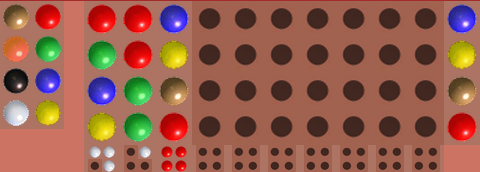
\includegraphics[width=.65\textwidth, keepaspectratio=true]{mm.png}
	    \end{center}
    \end{frame}

    \begin{frame}
    	\frametitle{Knuth Paper -- 1976}
    	\begin{enumerate}[label=\roman*.]
		\item At most five turns needed
		\end{enumerate}
%		\begin{tcolorbox}[colback=green!5,colframe=green!40!black,title=Minimax]
		For each possible guess
			\begin{enumerate}[label=]
			\item For each possible response to that guess
				\begin{enumerate}[label=]
				\item Check how many possible solutions remain
				\end{enumerate}
			\item Let \textit{score} be max. number solutions remaining
			\end{enumerate}
		Make guess with minimum score
%		\end{tcolorbox}
    \end{frame}
 
    \begin{frame}
    	\frametitle{Extensions}
		\begin{enumerate}[label=\roman*.]
		\item Basic Extension: $n$ spots, $k$ colors
		\item Repeats vs. no repeats
		\item Non-adaptive vs. adaptive strategies
		\end{enumerate}
    \end{frame}
    
    \begin{frame}
    \frametitle{Trivial Lower Bound}
    \begin{enumerate}[label=\arabic*.]
	\item One set of responses per solution
	\item \# of solutions = $k^n$
	\item $\binom{n+2}{2} \approx n^2$ responses per turn \\
	\onslide<2->{$\Rightarrow \binom{n+2}{2}^s \geq k^n$}
    \end{enumerate}
    \end{frame}

    \begin{frame}
    \frametitle{(Somewhat) Trivial Upper Bound}
    \begin{enumerate}[label=\arabic*.]
	\item Represent guesses and solutions as matrices ($Q_{ij} = 1$ iff the i-th spot is the j-th color)
	\item $Q_{ij} \in \mathbb R^{nk}$
	\item \# of black hits of $Q$ with hidden matrix $X$ is  $Q\cdot X$.
	\item Dot products with basis $\Rightarrow$ orthogonal basis \\
	$\Rightarrow$ Projections onto orthogonal basis $\Rightarrow$ X
    \end{enumerate}
    \end{frame}

    \begin{frame}
    \frametitle{Coin-Weighing Problem}
    [Grebinski \& Kucherov, 2000], [Bshouty, 2009]
    \begin{enumerate}[label=\roman*.]
		\item Original Coin-Weighing algorithm by G\&K, non-constructive (probabilistic method)
		\item Refined polynomial-time algorithm [Bshouty]
	\end{enumerate}
    [Doerr et. al., 2013]
    	\begin{enumerate}[label=\roman*.]
		\item Split hidden vector into ``coins'' (subvectors).
		\item ``Weight" of each ``coin" is \# of black hits.
		\item Use coin weighing algorithm to eliminate colors.
		\end{enumerate}
    \end{frame}

    \begin{frame}
    \frametitle{Entropy Method}
    \textit{Surprise Function:} For an event $x$, we want
	
    	\begin{enumerate}[label=\arabic*.]
		\item $S(x) = 0$ when $\mathbb{P}[x]=1$
		\item $S(x) = 1$ when $\mathbb{P}[x]=1/2$
		\item Decreasing function of $\mathbb{P}[x]$
		\item $S(x \land y)=S(x)+S(y|x)$\quad ($=S(x)+S(y)$ if independent)\\[2\baselineskip]
	\end{enumerate}

	\begin{enumerate}[label=]
	\item\onslide<2->{$\Rightarrow S(x)=-\log_2(\mathbb{P}[x])$.}
	\end{enumerate}
	\end{frame}
	
	\begin{frame}
	\frametitle{Entropy Method (cont'd)}
	Entropy is the expected surprise of a random variable.
	\textit{Definition:} Let $X$ be a random variable with domain $D$.
			\begin{equation*}
			H(X) = \sum_{x\in D}\mathbb{P}[X=x]\cdot(-\log_2\left(\mathbb{P}[X=x]\right))
			\end{equation*}
    \end{frame}
    
    \begin{frame}
    \frametitle{Probabilistic Method}
    Non-Adaptive Game: Set of queries $Q=\{q_1, q_2, \ldots, q_s\}$.
    	\begin{align*}
		\mathbb{P}[Q\text{ is a win} & \text{ning set of guesses }] > 0 \\
		& \Downarrow \\
		\exists \text{ a winning } & \text{set of $s$ guesses}
		\end{align*}
    \end{frame}

%    \begin{frame}
%    \frametitle{Future Topics to Explore}
%    \begin{enumerate}[label=\arabic*.]
%	\item $k>n$: no tight bounds
%	\item Permutation game algorithms
%	
%    \end{enumerate}
%    \end{frame}

\end{document}





























